\documentclass[11pt,a4paper]{article}
\usepackage[utf8]{inputenc}
\usepackage[francais]{babel}
\usepackage{amsmath}
\usepackage{amsfonts}
\usepackage{amssymb}
\usepackage{graphicx}
%\usepackage{fullpage}
\usepackage{placeins}
\usepackage{tabulary}
\usepackage{rotating}
\usepackage[font=small,labelfont=bf]{caption}
\author{Axel Struys - Alexis Buckens}
\title{Projet - Modèles linéaires}
\begin{document}
\maketitle
\section{Introduction}
Pour réaliser ce projet, nous avons choisi une base de données en provenance de l'UCI machine learning repository. Afin d'analyser les données, nous avons utilisé SAS university edition et R.
Ce dataset décrit plusieurs modèles de voitures en fonction de différentes caractéristiques. Plusieurs variables dépendantes pourraient être choisies pour ce dataset. Afin de restreindre notre analyse à une seule variable dépendante, nous avons choisi une question de recherche: "Quelles caractéristiques prédisent la consommation de carburant sur autoroute d'une voiture?".
Le dataset contenait à l'origine 26 variables: 16 continues et 10 nominales. Pour l'analyse, nous avons choisi 13 variables continues et 2 variables nominales. Nous avons exclu 4 variables continues car elles étaient des variables dépendantes. Nous avons exclu 8 variables nominales afin de simplifier le modèle. De plus, la variable highwaympg exprimait la consommation de carburant en miles par gallons. Afin d'exprimer cette consommation en unité européenne, nous l'avons transformée en L/100Km. Aussi, nous avons converti les unités de longueur en centimètres, les unités de poids en kilogrammes et les unités de volume en litres ($dm^{3}$).
Il y avait 205 observations à l'origine, mais pour 6 d'entre-elles, il y avait des valeurs manquantes. Nous avons supprimé ces observations. Le dataset ainsi nettoyé contient 199 observations.

Dans la table \ref{table:desc} nous présentons les statistiques descriptives pour les 13 variables continues, ainsi que les unités correspondantes. La table \ref{table:freq} présente les fréquences observées des deux variables discrètes : Aspiration et Engine type. Ces deux variables ont deux niveaux. On peut remarquer que les fréquences observées ne correspondent pas aux fréquences attendues: 40 observations par cellule. Pour l'analyse de la variance, nous sommes donc dans une situation où les cellules sont de tailles inégales. Il faudra donc adapter notre manière de calculer les effets principaux et les interactions pour ces deux variables discrètes.
Enfin, la table \ref{table:mean} présente la moyenne de consommation sur autoroute en fonction du type de carburant et du type d'aspiration d'air.
Ce tableau est représenté graphiquement sur la figure \ref{fig:meanauto}. De façon purement descriptive, on peut constater une consommation de carburation supérieure pour une aspiration de type turbo, ainsi qu'une consommation supérieure pour l'essence par rapport au diesel. Néanmoins,  nous devrons confirmer ces affirmation en testant les effets principaux de ces variables, ce que nous feront plus loin dans ce travail.


\begin{table}[ht]
	\centering
	\begin{tabular}{lrrrrr}
		\hline
		& mean & std.dev & median & min & max \\ 
		\hline
		wheelbase (cm) & 251.09 & 15.46 & 246.38 & 219.96 & 307.09 \\ 
		length (cm) & 442.21 & 31.72 & 439.93 & 358.39 & 528.57 \\ 
		width (cm) & 167.40 & 5.53 & 166.12 & 153.16 & 183.64 \\ 
		height (cm) & 136.69 & 6.08 & 137.41 & 121.41 & 151.89 \\ 
		curbweight (kg) & 1160.66 & 239.50 & 1094.97 & 674.94 & 1844.31 \\ 
		enginesize (L) & 2.10 & 0.68 & 1.97 & 1.00 & 5.34 \\ 
		bore (cm) & 8.45 & 0.70 & 8.41 & 6.45 & 10.01 \\ 
		stroke (cm) & 8.25 & 0.79 & 8.36 & 5.26 & 10.59 \\ 
		compressionratio & 10.17 & 4.03 & 9.00 & 7.00 & 23.00 \\ 
		horsepower (ch) & 104.15 & 40.05 & 95.00 & 48.00 & 288.00 \\ 
		peakrpm (tr/min) & 5107.79 & 467.59 & 5200.00 & 4150.00 & 6600.00 \\ 
		highwaylkm100 (L/100km) & 8.00 & 1.85 & 7.84 & 4.36 & 14.70 \\ 
		\hline
	\end{tabular}
\caption{Statistiques descriptives des 13 variables continues}
\label{table:desc}
\end{table}

\begin{table}[ht]
	\centering
	\begin{tabular}{llr}
		\hline
		Fueltype	& Aspiration & Count \\
		\hline
		 Diesel & Standard & 7 \\ 
		 Diesel & Turbo & 13 \\ 
		 Gas & Standard & 155 \\ 
		 Gas & Turbo & 24 \\ 
		\hline
	\end{tabular}
\caption{Fréquences observées pour les variables Aspiration \& Engine type}
\label{table:freq}
\end{table}
\begin{table}[ht]
	\centering
	\begin{tabular}{llr}
		\hline
		Fueltype & Aspiration & highwaylkm100.mean \\ 
		\hline
		Diesel & Standard & 5.44 \\ 
		Diesel & Turbo & 8.11 \\ 
		Gas & Standard & 7.90 \\ 
		Gas & Turbo & 9.37 \\ 
		\hline
	\end{tabular}
\caption{Moyenne de la consommation (L/100km) en fonction du type de carburant et de l'aspiration}
\label{table:mean}
\end{table}

\begin{figure}
	\centering
	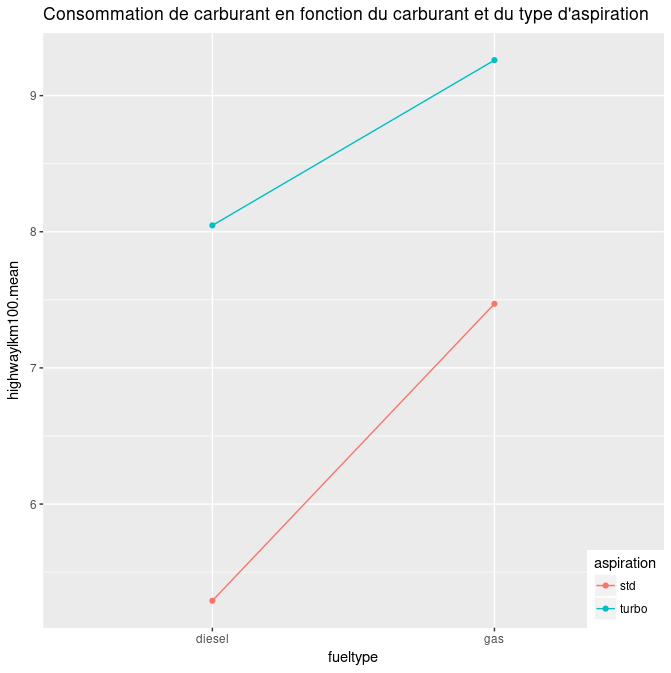
\includegraphics[width=0.8\linewidth]{meanauto}
	\caption{Moyenne de la consommation (L/100km) en fonction du type de carburant et de l'aspiration}
	\label{fig:meanauto}
\end{figure}

\section{Sélection du modèle de régression}

\subsection{Multicolinéarité}

Afin de sélectionner un bon modèle de régression, il faut en premier lieu éviter la multicolinéarité. Celle-ci est mesurée par le VIF (variance inflation factor). Celui-ci indique à quel point une variable augmente artificiellement la somme des carrés du modèle. Aussi, c'est une mesure de la corrélation de la variable avec les autres variables du modèle. Une variable est donc redondante si la proportion de la variance qu'elle explique est aussi expliquée par une autre variable du modèle. Si cette proportion est trop grande, alors il est utile de supprimer cette variable indépendante afin de simplifier le modèle. En termes d'algèbre linéaire, c'est une mesure de la dépendance linéaire entre les variables. Si une variable est linéairement dépendante d'une autre, l'inversion de la matrice devient impossible. Dans ce cas, il n'est pas possible de calculer les termes de la régression. Plus une variable se rapproche de la dépendance linéaire, et plus le modèle devient instable.
Un critère pour la grandeur VIF est qu'aucune variable ne peut avoir un VIF supérieur à 10. De plus, la moyenne des VIF ne doit pas être  grandement supérieure à 1.

Nous avons lancé un premier modèle via SAS en incluant toutes les variables afin de vérifier la multicolinéarité. La table \ref{table:firstreg} montre que curbweight, enginesize et horsepower ont un VIF supérieur à / proche de 10. En réalisant un corrélation sur toutes les variables numériques (voir table \ref{table:corrvif} en annexe) on remarque que curbweight, enginesize et horsepower sont fortement corrélées entre elles. De plus, elles sont corrélées avec les autres variables. Ces corrélations font sens d'un point de vue théorique, étant donné que la puissance d'un moteur est directement liée à son volume. Néanmoins, horsepower est en moyenne moins corrélées avec les autres variables que les deux premières variables, et son VIF est plus petit. Nous allons donc supprimer ces deux variables, et garder horsepower. En réalisant à nouveau une régression, on constate que tous les VIF sont inférieurs à 10, et que le VIF moyen est de $3,363$. On peut considérer ceci comme acceptable.
%préciser vif (formule math) + preciser multicolinéarité

\begin{table}
\small
	\begin{tabulary}{1\textwidth}{LRRRRRR}\hline
		\multicolumn{7}{c}{Parameter Estimates}\\\hline
		Variable &    DF &    Parameter  Estimate &    Standard  Error &    t~Value &    $Pr ~>~ |t|$ &    Variance  Inflation\\\hline
		
	Intercept &    1 &    $-$2.68801 &    2.81974 &    $-$0.95 &    0.3417 &    0\\\hline
	wheelbase &    1 &    $-$0.00454 &    0.00765 &    $-$0.59 &    0.5537 &    7.51130\\\hline
	length &    1 &    0.00685 &    0.00407 &    1.68 &    0.0938 &    8.93723\\\hline
	width &    1 &    0.00656 &    0.01855 &    0.35 &    0.7241 &    5.64192\\\hline
	height &    1 &    0.01087 &    0.01079 &    1.01 &    0.3151 &    2.31344\\\hline
	curbweight &    1 &    0.00381 &    0.00067915 &    5.61 &    $<$.0001 &    14.19486\\\hline
	enginesize &    1 &    1.55782 &    0.20856 &    7.47 &    $<$.0001 &    10.80793\\\hline
	bore &    1 &    $-$0.19462 &    0.09008 &    $-$2.16 &    0.0320 &    2.11806\\\hline
	stroke &    1 &    $-$0.23587 &    0.06268 &    $-$3.76 &    0.0002 &    1.32045\\\hline
	horsepower &    1 &    $-$0.00822 &    0.00337 &    $-$2.44 &    0.0158 &    9.79074\\\hline
	peakrpm &    1 &    0.00048201 &    0.00013387 &    3.60 &    0.0004 &    2.10236\\\hline
	fueldummy &    1 &    $-$1.09864 &    0.10096 &    $-$10.88 &    $<$.0001 &    1.98744\\\hline
	aspirationdummy &    1 &    0.58015 &    0.08188 &    7.09 &    $<$.0001 &    2.18891\\\hline
	\end{tabulary}

\caption{Premier modèle incluant tous les facteurs: on peut voir que curbweight, enginesize et horsepower ont un vif supérieur à / proche de 10.}
\label{table:firstreg}
\end{table}

\subsection{Méthodes de sélections du modèle de régression}

Après avoir vérifié la multicolinéarité, plusieurs méthodes sont disponibles afin de sélectionner les variables à inclure dans le modèle final. 

\paragraph{Méthodes de type 1} Il est possible de choisir le meilleur modèle parmi tous les modèles possibles, sur base d'un critère; Nous comparerons ici le critère de Mallows et le critère du coefficient de détermination ajusté. Grâce à SAS, nous pouvons rapidement calculer le meilleur modèles. Un inconvénient majeur de ces méthodes est que plus le nombre de variables dans le modèle augmente, plus cela demande de ressources de calcul étant donné que le logiciel doit calculer toutes les permutations possibles. Dans notre cas, le nombre de variable de bases est raisonnable, ce qui permet l'emploi de ces méthodes.
%2 tables pour comparer les deux critères -> annexe
Les tables \ref{table:mallows} et \ref{table:adjsqr} permettent de comparer les 5 meilleurs modèles en fonction de ces deux critères. En fonction du critère de Mallows, dont l'estimateur est C(p), le meilleur modèle ne contient que 6 variables, et explique 81\% de la variance. En utilisant le critère du R$^2$ ajusté, le meilleur modèle contient 8 variables, et explique aussi 81\% de la variance. Néanmoins, il nous semble plus pertinent d'être parcimonieux dans le nombre de variables explicatives à inclure. Dans ce cas, le modèle incluant 6 variables est plus intéressant. On pourrait même considérer le quatrième meilleur modèle selon le critère de Mallows, qui ne contient que 5 variables et pourtant explique toujours 81\% de la variance.

\begin{table}
	\small
\begin{tabulary}{1\textwidth}{LlLJ}
	\hline

	Number in Model &    C(p) &    R-Square &    Variables in Model\\\hline
	
	6 &    7.8733 &    0.8152 &    wheelbase length width horsepower fueldummy aspirationdummy\\
	7 &    8.2218 &    0.8168 &    wheelbase length width horsepower peakrpm fueldummy aspirationdummy\\
	8 &    8.5198 &    0.8184 &    wheelbase length width bore horsepower peakrpm fueldummy aspirationdummy\\
	5 &    9.0007 &    0.8122 &    wheelbase length horsepower fueldummy aspirationdummy\\
	7 &    9.1320 &    0.8159 &    wheelbase length width bore horsepower fueldummy aspirationdummy\\\hline
	
\end{tabulary}

\caption{Sélection des 5 meilleurs modèles en fonction du critère de Mallows (C(p)).}
\label{table:mallows}
\end{table}

\begin{table}
\small
\begin{tabulary}{1\textwidth}{LLLJ}\hline
	
	Number in  Model &    Adjusted  R-Square &    R-Square &    Variables in Model\\\hline

	  8 &    0.8108 &    0.8184 &    wheelbase length width bore horsepower peakrpm fueldummy aspirationdummy\\
	9 &    0.8108 &    0.8194 &    wheelbase length width bore stroke horsepower peakrpm fueldummy aspirationdummy\\
	10 &    0.8103 &    0.8199 &    wheelbase length width height bore stroke horsepower peakrpm fueldummy aspirationdummy\\
	7 &    0.8101 &    0.8168 &    wheelbase length width horsepower peakrpm fueldummy aspirationdummy\\
	9 &    0.8100 &    0.8187 &    wheelbase length width height bore horsepower peakrpm fueldummy aspirationdummy\\\hline
	
\end{tabulary}
\caption{Sélection des 5 meilleurs modèles en fonction du critère du R$^2$}
\label{table:adjsqr}
\end{table}


\paragraph{Méthodes de type 2}Une deuxième approche est d'inclure ou exclure séquentiellement des variables du modèle. Plusieurs méthodes sont disponibles: forward selection, backward elimination, forward stepwise, etc... Un avantage de ces méthodes est qu'elles sont plus économiques en termes de temps de calcul pour l'ordinateur. Dans le cas d'une inclusion séquentielle, on commence avec la variable indépendante qui explique le plus la variable dépendante (Le plus grand R$^{2}$). Ensuite, on va ajouter séquentiellement des variables, toujours en utilisant ce critère, jusqu'à atteindre le significance level to stop : la p valeur de la variable ajoutée est plus grande qu'une p valeur déterminée. Dans le cas d'une backward élimination, on commence avec toutes les variables, et on supprime séquentiellement. Pour une selection stepwise, on recalcule à chaque étape si on peut supprimer une variable précédemment ajoutée. Nous allons comparer ces trois techniques. Pour la méthode forward selection, nous avons choisi un seuil d'entrée de 0.1. Pour la méthode backward élimination, nous avons choisi un seuil d'élimination de 0.15. Enfin, pour la méthode forward stepwise, les seuils d'entrée et d'élimination étaient de 0.1 et 0.15 respectivement. Dans les tables \ref{table:forward}, \ref{table:backward} et \ref{table:stepwise} en annexe, on peut constater que les 3 méthodes convergent vers la même solution: les variables heigth, stroke, bore et peakrpm sont éliminées, tandis que horsepower, length, fuel, wheelbase, aspiration et width sont conservées. Remarquons que ces méthodes proposent les mêmes 6 variables que le meilleur modèle selon le critère de Mallows.
%préciser ce passage avec le livre
%inclure les 3 tables en annexe

\begin{table}
	\scriptsize
	\centering
	\begin{tabulary}{1\textwidth}{LLLLLlLL}
	  \multicolumn{8}{c}{Summary of Forward Selection}\\\hline
	Step &    Variable {\newline} Entered &    Number Vars In &    Partial R-Sq &    Model R-Sq &    C(p) &    F Value &    $Pr~>~F$\\\hline
	1 &    horsepower &    1 &    0.6579 &    0.6579 &    162.071 &    378.80 &    $<$.0001\\
	2 &    length &    2 &    0.1155 &    0.7734 &    43.5431 &    99.87 &    $<$.0001\\
	3 &    fueldummy &    3 &    0.0234 &    0.7967 &    21.1259 &    22.45 &    $<$.0001\\
	4 &    wheelbase &    4 &    0.0105 &    0.8073 &    12.1210 &    10.62 &    0.0013\\
	5 &    aspirationdummy &    5 &    0.0049 &    0.8122 &    9.0007 &    5.04 &    0.0259\\
	6 &    width &    6 &    0.0030 &    0.8152 &    7.8733 &    3.11 &    0.0792\\\hline

	\end{tabulary}
	\caption{Résumé de la méthode de Forward selection : 6 variables sont retenues au seuil $p~<~0.1$.}
	\label{table:forward}
\end{table}

\begin{table}
	\scriptsize
	\centering
	\begin{tabulary}{1\textwidth}{LLLLLLLL}
		
		\multicolumn{8}{c}{Summary of Backward Elimination}\\\hline
		Step &    Variable {\newline} Removed &    Number  Vars In &    Partial  R-Sq &    Model {\newline} R-Sq &    C(p) &    F Value &    $Pr~>~F$\\\hline
	
		1 &    height &    9 &    0.0005 &    0.8194 &    9.5281 &    0.53 &    0.4683\\
		2 &    stroke &    8 &    0.0010 &    0.8184 &    8.5198 &    0.99 &    0.3200\\
		3 &    bore &    7 &    0.0016 &    0.8168 &    8.2218 &    1.71 &    0.1930\\
		4 &    peakrpm &    6 &    0.0016 &    0.8152 &    7.8733 &    1.65 &    0.2006\\\hline
	\end{tabulary}
	\caption{Résumé de la méthode de Backward elimination : 4 variables sont supprimées au seuil $p ~>~ 0.15$}
	\label{table:backward}
\end{table}

\begin{table}
	\scriptsize
	
	\begin{tabulary}{1\textwidth}{LLLLLLlll}
	
		   \multicolumn{9}{c}{Summary of Stepwise Selection}\\\hline
		Step &    Variable Entered &    Variable Removed &    Number Vars In &    Partial  R-Sq &    Model  R-Sq &    C(p) &    F Value &    $Pr>F$\\\hline

		1 &    horsepower &      &    1 &    0.6579 &    0.6579 &    162.07 &    378.80 &    $<$.0001\\
		2 &    length &      &    2 &    0.1155 &    0.7734 &    43.54 &    99.87 &    $<$.0001\\
		3 &    fueldummy &      &    3 &    0.0234 &    0.7967 &    21.12 &    22.45 &    $<$.0001\\
		4 &    wheelbase &      &    4 &    0.0105 &    0.8073 &    12.12 &    10.62 &    0.0013\\
		5 &    aspirationdummy &      &    5 &    0.0049 &    0.81 &    9.0007 &    5.04 &    0.0259\\
		6 &    width &      &    6 &    0.0030 &    0.8152 &    7.87 &    3.11 &    0.0792\\\hline
	\end{tabulary}
	\caption{Résumé de la méthode stepwise forward selection : 6 variables sont retenues au seuil de sélection $p~<0.1$, et aucune variable n'est retirée au seuil $p~>~0.15$}
	\label{table:stepwise}
\end{table}

\paragraph{Méthodes de type 3} Ce type de méthodes est utile lorsque le nombre de variables dans le modèle est très grand. Nous allons utiliser la méthode LASSO vue au cours, via SAS. Ici aussi, l'étape optimale retient les même 6 variables que précédemment.

\begin{table}
	\scriptsize
	\centering
	\begin{tabulary}{1\textwidth}{LLLLL}
	\hline
	   \multicolumn{5}{c}{LASSO Selection Summary}\\\hline
	Step &    Effect {\newline} Entered &    Effect {\newline} Removed &    Number {\newline} Effects In &    BIC \\\hline
	0 &    Intercept &      &    1 &    245.4286\\
	1 &    horsepower &      &    2 &    188.7603\\
	2 &    length &      &    3 &    117.5676\\
	3 &    width &      &    4 &    $-$22.4925\\
	4 &    fueldummy &      &    5 &    $-$22.8460\\
	5 &    wheelbase &      &    6 &    $-$64.1505\\
	6 &    aspirationdummy &      &    7 &    $-$71.8419*\\
	7 &    peakrpm &      &    8 &    $-$71.8178\\
	8 &    stroke &      &    9 &    $-$71.5047\\
	9 &    bore &      &    10 &    $-$70.8762\\
	10 &    height &      &    11 &    $-$71.4571\\\hline
	\multicolumn{5}{c}{*~Optimal~Value~of~Criterion}\\\hline
	\end{tabulary}
	\caption{Sélection lasso. Le step optimal est le 6\ieme{}.}
	\label{table:lasso}
\end{table}

\paragraph{Modèle sélectionné} Les différentes méthodes que nous avons présenté convergent vers le même modèle à sélectionner, contenant 6 variables.

\begin{table}
	\scriptsize
	\centering
	\begin{tabulary}{1\textwidth}{LLLLLL}
	   \multicolumn{6}{c}{Analysis of Variance}\\\hline
	Source &    DF &    Sum of  Squares &  Mean Square &    F Value &    $Pr~>~F$\\\hline

	Model &    6 &    553.85484 &    92.30914 &    141.16 &    $<$.0001\\
	Error &    192 &    125.55930 &    0.65395 &      &     \\
	Corrected Total &    198 &    679.41413 &      &      &     \\\hline
	\end{tabulary}
	\newline
	\vspace{5mm}
	\newline
	\begin{tabulary}{1\textwidth}{LL|LL}
		\hline
		Root MSE &    0.80867 &    R-Square &    0.8152\\
		Dependent Mean &    8.00271 &    Adj R-Sq &    0.8094\\
		Coeff Var &    10.10501 &      &     \\\hline
	\end{tabulary}
	\newline
	\vspace{5mm}
	\newline
	\begin{tabulary}{1\textwidth}{LLLLLL}
	\multicolumn{6}{c}{Parameter Estimates}\\\hline
	Variable &    DF &    Parameter  Estimate &    Standard  Error &    t~Value &    Pr$~>~|t|$\\\hline
	Intercept &    1 &    $-$13.19524 &    2.75453 &    $-$4.79 &    $<$.0001\\
	wheelbase &    1 &    0.01934 &    0.00913 &    2.12 &    0.0354\\
	length &    1 &    0.01492 &    0.00466 &    3.20 &    0.0016\\
	width &    1 &    0.04188 &    0.02374 &    1.76 &    0.0792\\
	horsepower &    1 &    0.02182 &    0.00239 &    9.14 &    $<$.0001\\
	fueldummy &    1 &    $-$0.72761 &    0.11985 &    $-$6.07 &    $<$.0001\\
	aspirationdummy &    1 &    0.19410 &    0.08603 &    2.26 &    0.0252\\\hline
	\end{tabulary}

	\caption{Résumé du modèle final sélectionné}
	\label{table:aov}
\end{table}

\section{Diagnostic du modèle linéaires et mesures correctrices}
\subsection{Diagnostic}
Nous allons maintenant nous intéresser à la vérification des hypothèses sous-jascentes à la regression.
Il y a trois principales hypothèses: l'homoscédasticité, la normalité des résidus et l'indépendance des observations. De plus, des observation aberrantes et influentes peuvent influencer la construction du modèle de régression. Les figures \ref{fig:diagnostics} et\ref{fig:regressors} présentent les différents graphes nous permettant de répondre à ces questions.

\paragraph{Homoscédasticité} Nous pouvons répondre à cette question en observant le graphe des résidus par rapport aux valeurs prédites. Nous pouvons voir que les erreurs se répartissent aléatoirement autour de 0, indiquant une variance homogène. Il n'y a pas de structure claire se dégageant du graphe.
Néanmoins, sur la figure \ref{fig:regressors}, nous constatons que la variance des deux variables catégorielles est différente pour chaque niveau. Il y a un problème d'héteroskédasticité pour ces deux variables catégorielles.
%test homoscé%
\paragraph{Normalité des résidus} Le Q-Q plot nous permet de comparer les quantiles de notre distribution aux quantiles de la distribution normale. Si tous les points sont sur la diagonale, alors notre distribution est normale. Nous pouvons constater que les résidus sont en moyenne situés sur la droite. Néanmoins, les valeurs extrêmes de la distribution s'écartent de la distribution normale. Sur l'histogramme des résidus, nous pouvons voir que leur densité se rapproche d'une normale. Nous pouvons donc faire l'hypothèse, prudente, que les résidus suivent une distribution normale.
%testnormalité%
\paragraph{Indépendance des observation} D'un point de vue théorique, chaque modèle de voiture de ce dataset est différent. Néanmoins, il faut être prudent avec cette affirmation. En effet, il est raisonnable de penser qu'un constructeur produisant plusieurs modèle de voiture réutilise certains composants dans différents modèles, offrant des performances similaires. Dans ce cas, il pourrait exister des observations qui ne sont pas indépendantes les unes des autres. Via SAS, nous avons réalisé un test de Durbin-Watson pour l'autocorrélation. Celui-ci indique une autocorrélation positive signification de premier ordre de 0.288.
\begin{table}
	\scriptsize
	\centering
	\begin{tabulary}{1\textwidth}{LL}
		\hline
		 Durbin-Watson D &    1.406\\
		$Pr < DW$ &    $<$.0001\\
		$Pr > DW $&    1.0000\\
		Number of Observations &    199\\
		1st Order Autocorrelation &    0.288\\\hline
	\end{tabulary}
	\caption{Test de Durbin-Watson pour l'autocorrélation}
	\label{table:}
\end{table}
% ajouter tests d'autocorrélation d'obs%
\paragraph{Observations aberrantes}
Sur le graphe ... nous pouvons observer les leviers par rapport au numéro d'observation. C'est une mesure des observations aberrantes par rapport aux régresseurs.
Sur le graphe ... nous pouvons observer les résidus effacés studentisés par rapport au numéro d'observation. C'est une mesure des observations aberrantes par rapport  à la réponse.

\paragraph{Observations influentes} Le graphe des DFFITS (figure ...) permet d'observer les observations influentes par rapport aux valeurs prédites
Le graphe des distances de Cook (figure ...) permet de détecter la présence d'observations influentes sur les valeurs prédites, ainsi que sur les coefficients de la régression.

\subsection{Mesures correctrices}
\paragraph{Correction de l'heteroskedasticité et de l'autocorrélation}
Nous avons vu que la variance des variables catégorielles n'était pas homogène. En outre, il y avait une autocorrélation de premier ordre significative. Elle était certes faible, mais nous avons voulu la corriger. Comme suggéré précédemment, la non-indépendance provient peut-être du fait que les différents modèles de voiture provenant d'un même constructeur ont des caractéristiques similaires. Comme suggéré par Neter(2004), une solution possible à cette autocorrélation est d'inclure des variables indépendantes susceptibles d'être la source de cette non indépendance. Ainsi, nous avons relancé un modèle en ajoutant les modèles de voitures comme variables indépendantes. De plus, afin de corriger l'hétéroscédasticité, nous avons réalisé une transformation de box-cox sur la variable dépendantes.

\paragraph{Correction des observations influentes et aberrantes}
...


\paragraph{Modèle final après corrections}
Sur le graphe ... nous pouvons constater que les variances des prédicteurs catégoriels est maintenant beaucoup plus homogène.
De plus, le test de Durbin-Watson pour l'autocorrélation nous montre que celle-ci à été fortement réduite, passant a 0.054. Néanmoins, elle est toujours significative, indiquant qu'il existe toujours une petite source d'autocorrélation, non-identifiée.


\begin{table}
	\scriptsize
	\centering
	\begin{tabulary}{1\textwidth}{LL}\hline
		Durbin-Watson D &    1.888\\
		$Pr < DW$ &    0.0122\\
		$Pr > DW$ &    0.9878\\
		Number of Observations &    199\\
		1st Order Autocorrelation &    0.054\\\hline
	\end{tabulary}
	\caption{Test de Durbin-Watson après correction via ajout des constructeurs de voitures comme variables de contrôle.}
	\label{table:dwcorrected}
\end{table}

\begin{figure}
	\centering
	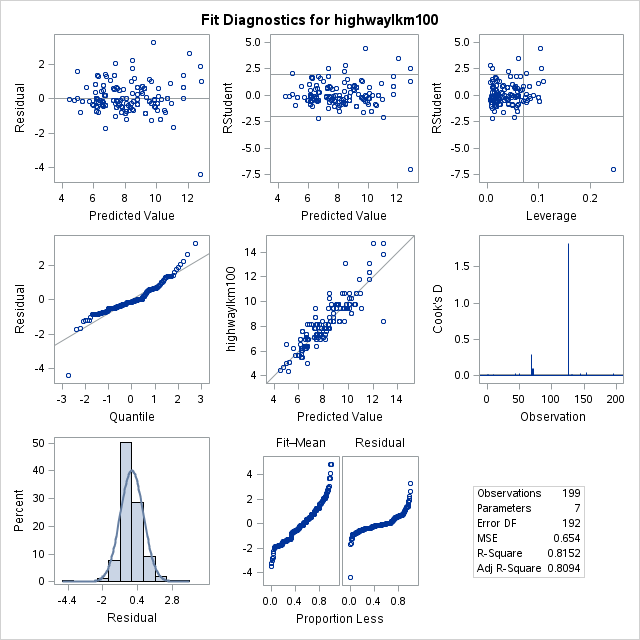
\includegraphics[width=1\linewidth]{fitdiagnostics}
	\caption{Résumé des différents diagnostiques du modèle de régression}
	\label{fig:diagnostics}
\end{figure}
\begin{figure}
	\centering
	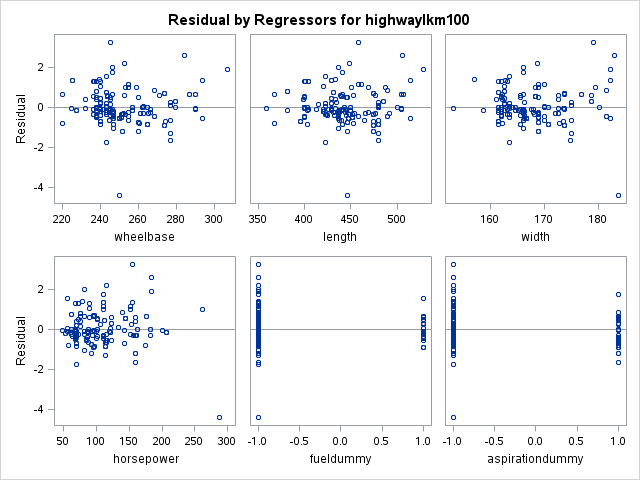
\includegraphics[width=1\linewidth]{resbyregressors}
	\caption{Graphes des résidus par régresseurs}
	\label{fig:regressors}
\end{figure}

\section{Prédiction}

On peut également tenter de calculer l'intervalle de prédiction sur une nouvelle valeur. La première étape consiste à choisir cette nouvelle valeur sur laquelle estimer l'intervalle. Pour ce faire, on peut demander à l'ordinateur de générer une nouvelle variable avec une distribution de moyenne et variance égale à celle de chacune des variables. 

Si on calcule l'intervalle de prédiction sur une nouvelle donnée construite par cette méthode, on obtient une valeur prédite de 6.577 et un intervalle compris entre 4.86 et 8.29. Si les valeurs semblent à priori raisonnables (elles ne sont en effet pas très éloignées de la moyenne de la variable dépendante), il peut néanmoins être frustrant de constater la largeur de l'intervalle de prédiction. La borne supérieure est en effet près du double de la borne inférieure (1.7 fois celle-ci exactement). La largeur de cet intervalle est peut-être normal, mais il est intéressant de se poser la question de ce qui a pu aller de travers et provoquer cet intervalle qui semble excessivement large.

Si on considère que cet intervalle large n'est pas naturel et provient d'une erreur dans le modèle, on peut rechercher d'où provient ce résultat. On pourrait penser que la transformation, en modifiant les unité pourrait être à l'origine de cet écart démesuré. Néanmoins, la même technique appliquée aux unités d'origine donne un résultat similaire au résultat obtenu précédemment.

\section{Annexes}
\appendix
\section{Vérification des VIF}
\begin{table}
	\scriptsize
	\centering
	\begin{tabulary}{1\textwidth}{|L|R|R|R|R|R|R|R|R|R|R|}
	\hline
 &    wheelbase &    length &    width &    height &    curbweight &    enginesize &    bore &    stroke &    horsepower &    peakrpm\\\hline

wheelbase &    1.00 &    0.88 &    0.80 &    0.59 &    0.78 &    0.57 &    0.49 &    0.17 &    0.36 &    $-$0.35\\\hline
length &    0.88 &    1.00 &    0.84 &    0.50 &    0.88 &    0.69 &    0.61 &    0.12 &    0.56 &    $-$0.28\\\hline
width &    0.80 &    0.84 &    1.00 &    0.29 &    0.87 &    0.75 &    0.56 &    0.18 &    0.64 &    $-$0.22\\\hline
height &    0.59 &    0.50 &    0.29 &    1.00 &    0.30 &    0.03 &    0.18 &    $-$0.05 &    $-$0.11 &    $-$0.28\\\hline
curbweight &    0.78 &    0.88 &    0.87 &    0.30 &    1.00 &    0.86 &    0.65 &    0.17 &    0.75 &    $-$0.27\\\hline
enginesize &    0.57 &    0.69 &    0.75 &    0.03 &    0.86 &    1.00 &    0.59 &    0.21 &    0.83 &    $-$0.21\\\hline
bore &    0.49 &    0.61 &    0.56 &    0.18 &    0.65 &    0.59 &    1.00 &    $-$0.07 &    0.58 &    $-$0.26\\\hline
stroke &    0.17 &    0.12 &    0.18 &    $-$0.05 &    0.17 &    0.21 &    $-$0.07 &    1.00 &    0.09 &    $-$0.07\\\hline
horsepower &    0.36 &    0.56 &    0.64 &    $-$0.11 &    0.75 &    0.83 &    0.58 &    0.09 &    1.00 &    0.13\\\hline
peakrpm &    $-$0.35 &    $-$0.28 &    $-$0.22 &    $-$0.28 &    $-$0.27 &    $-$0.21 &    $-$0.26 &    $-$0.07 &    0.13 &    1.00\\\hline

	
\end{tabulary}
			\caption{Corrélations entre les variables numériques: on remarque que curbweigth, enginesize et horsepower sont fortement corrélées entre elles}
			\label{table:corrvif}
		\end{table}
\end{document}